\documentclass[runningheads]{llncs}
\usepackage{graphicx}
\usepackage{amsmath,amssymb}
\usepackage{booktabs}
\usepackage{multirow}
\usepackage{xcolor}
\usepackage{tikz}
\usetikzlibrary{positioning,arrows.meta,fit,calc}
\usepackage{subcaption}
\usepackage{hyperref}

\definecolor{dyncolor}{RGB}{66,133,244}
\definecolor{fixcolor}{RGB}{52,168,83}
\definecolor{newcolor}{RGB}{251,188,4}
\definecolor{tempcolor}{RGB}{171,71,188}

\newcommand{\ie}{\emph{i.e.}}
\newcommand{\eg}{\emph{e.g.}}
\newcommand{\etal}{\emph{et al.}}

\sloppy
\begin{document}

\title{NC-Conv: Noise-Conditioned Dual-Path Convolution\\for Degradation-Robust Vision}

\titlerunning{NC-Conv: Noise-Conditioned Dual-Path Convolution}

\author{Anonymous ACCV 2026 submission}
\authorrunning{Anonymous}
\institute{Anonymous}

\maketitle

% ============================================================
\begin{abstract}
We present \textbf{NC-Conv}, a noise-conditioned dual-path convolution that transfers the audio noise-conditioning framework to vision.
Each NC-Conv block blends a \textcolor{fixcolor}{\emph{static}} path (fixed weights, $O(\sigma_n^2)$ noise variance) with a \textcolor{dyncolor}{\emph{dynamic}} path (input-dependent modulation, $O(\sigma_n^{4+})$) via a learned quality gate $\sigma$: clean inputs activate the expressive dynamic path ($\sigma{\approx}1$), while degraded inputs fall back to the robust static path ($\sigma{\approx}0$).
On the CIFAR-10-C benchmark (19 corruptions $\times$ 5 severities), NC-Conv achieves \textbf{+1.6\%} average accuracy over a parameter-matched standard CNN, with the advantage scaling monotonically from $+0.5\%$ at severity~1 to $\mathbf{+2.9\%}$ at severity~5---directly validating the noise propagation theory.
On CULane lane detection, NC-Conv achieves $+6.5\%$ on normal and $\mathbf{+21.7\%}$ on fog conditions.
For video, a \textcolor{tempcolor}{bidirectional temporal NC-SSM} with per-frame quality gating recovers $\mathbf{+35.2\%}$ accuracy on the darkest tunnel frame while preserving clean-frame accuracy within $1\%$.
At 253K parameters (deployable on a \$8 MCU), NC-Conv establishes noise-conditioned computation as a modality-agnostic framework for degradation-robust edge perception.

\keywords{Corruption robustness, Noise conditioning, Dynamic convolution, Lane detection, State space models, Edge AI}
\end{abstract}

% ============================================================
\section{Introduction}
\label{sec:intro}

Deep vision models degrade significantly under adverse conditions---fog, low light, noise, and compression artifacts---precisely when robust perception is most critical for safety applications such as autonomous driving and surveillance.
While corruption augmentation during training improves robustness, it treats all inputs identically regardless of quality, missing the opportunity to adapt processing to the specific degradation level.

We draw inspiration from \emph{audio noise robustness}.
In keyword spotting, our prior work~\cite{choi2026ncssm} showed that selective state space models (SSMs) with input-dependent dynamics amplify noise as $O(\sigma_n^6)$, while fixed (LTI) systems maintain $O(\sigma_n^2)$.
The NC-SSM solution---blending selective and fixed dynamics based on local signal quality---transfers to CNNs when we observe that \emph{input-dependent channel modulation} (SE-Net~\cite{hu2018squeeze}, dynamic convolution~\cite{chen2020dynamic}) creates analogous multiplicative noise amplification:
\begin{equation}
h = \alpha(x) \odot \text{Conv}(x) \implies \text{Var}[h] = O(\sigma_n^{4+}).
\end{equation}
A fixed convolution without input-dependent modulation maintains $\text{Var}[h] = O(\sigma_n^2)$.

\textbf{NC-Conv} provides a principled solution: blend dynamic (expressive, noise-sensitive) and static (robust, less expressive) convolutional paths via a learned quality gate $\sigma$ that automatically adapts to input degradation level.
For video sequences with temporally varying degradation (\eg, tunnel entry/exit), we add a \textbf{bidirectional temporal NC-SSM} that enables clean-frame context to propagate to degraded frames.

\noindent\textbf{Contributions.}
\begin{enumerate}
\setlength\itemsep{0pt}
\item \textbf{NC-Conv block}: Dual-path convolution with learned $\sigma$ gate providing noise-conditioned routing between expressive and robust paths (\S\ref{sec:method}).
\item \textbf{Severity scaling}: On CIFAR-10-C, NC-Conv's advantage grows monotonically with corruption severity ($+0.5\%$ to $+2.9\%$), directly validating the noise propagation theory (\S\ref{sec:cifar10c}).
\item \textbf{Bidirectional temporal NC-SSM}: Per-frame quality-gated temporal dynamics enable clean-to-degraded context transfer, recovering $+35.2\%$ on tunnel interiors (\S\ref{sec:temporal_exp}).
\item \textbf{Real-world validation}: On CULane lane detection, NC-Conv achieves $+21.7\%$ on fog and $+6.5\%$ on normal conditions (\S\ref{sec:culane}).
\item \textbf{Per-spatial $\sigma$}: Extension from per-sample to per-spatial quality maps addresses impulse noise limitation ($+1.0\%$) (\S\ref{sec:spatial_sigma}).
\end{enumerate}


% ============================================================
\section{Related Work}
\label{sec:related}

\noindent\textbf{Corruption robustness.}
The CIFAR-10-C/ImageNet-C benchmarks~\cite{hendrycks2019benchmarking} standardized corruption robustness evaluation.
AugMix~\cite{hendrycks2020augmix} and DeepAugment~\cite{hendrycks2021deepaugment} improve robustness through diverse augmentation but apply uniform processing regardless of input quality.
NC-Conv combines augmentation with \emph{quality-adaptive} dual-path routing.

\noindent\textbf{Dynamic and conditional computation.}
Dynamic convolution~\cite{chen2020dynamic} uses input-dependent kernel attention; SE-Net~\cite{hu2018squeeze} provides channel recalibration.
Conditional computation~\cite{bengio2013estimating} routes inputs through different sub-networks.
NC-Conv uniquely grounds dual-path routing in \emph{noise propagation theory}, providing a principled static fallback under degradation.

\noindent\textbf{Noise-conditioned SSMs.}
Our audio NC-SSM~\cite{choi2026ncssm} blends selective ($O(\sigma_n^6)$) and LTI ($O(\sigma_n^2)$) SSM dynamics per sub-band based on SNR.
NC-Conv extends this principle to CNNs (spatial) and conv1d-based SSMs (temporal).


% ============================================================
\section{Method: NC-Conv}
\label{sec:method}

\subsection{Noise Propagation in CNNs}
\label{sec:theory}

\noindent\textbf{Definition 1 (Static and Dynamic Convolution).}
Let $x \in \mathbb{R}^{C \times H \times W}$ be an input feature map.
A \textbf{static} convolution computes $h_s = W * x$ with fixed kernel $W$.
A \textbf{dynamic} convolution computes $h_d = (W * x) \odot \alpha(x)$, where $\alpha(x) = \text{Sigmoid}(\text{FC}(\text{GAP}(x)))$ is a channel-wise input-dependent gate.

\noindent\textbf{Proposition 1 (Static Noise Variance).}
For noisy input $x = s + n$, $n \sim \mathcal{N}(0, \sigma_n^2 I)$, and fixed kernel $W$:
$\text{Var}[h_s] = \|W\|_F^2 \cdot \sigma_n^2 = O(\sigma_n^2).$

\noindent\textbf{Proposition 2 (Dynamic Noise Amplification).}
For the dynamic path $h_d = (W * x) \odot \alpha(x)$:
\begin{equation}
\text{Var}[h_d] = \underbrace{O(\sigma_n^2)}_{\text{conv}} + \underbrace{O(\sigma_n^4)}_{\text{cross}} + \underbrace{O(\sigma_n^6)}_{\text{triple}}.
\label{eq:dynamic_var}
\end{equation}
The multiplicative coupling $\alpha(x) \odot (W{*}x)$ creates cross-terms analogous to the $O(\sigma_n^6)$ bound for selective SSMs~\cite{choi2026ncssm}.

Table~\ref{tab:noise_parallel} summarizes the correspondence: \emph{any} input-dependent parameterization creates multiplicative noise coupling, regardless of whether the underlying operation is an SSM recurrence or a convolutional gate.

\begin{table}[t]
\centering
\caption{Noise variance by operation type.}
\label{tab:noise_parallel}
\small
\begin{tabular}{@{}lcc@{}}
\toprule
\textbf{Operation} & \textbf{Audio (SSM)} & \textbf{Vision (CNN)} \\
\midrule
Fixed (input-indep.) & LTI: $O(\sigma_n^2)$ & Static Conv: $O(\sigma_n^2)$ \\
Input-dependent & Selective: $O(\sigma_n^6)$ & Dynamic: $O(\sigma_n^{4+})$ \\
\textbf{NC (ours)} & $O(\sigma_n^{2+\epsilon})$ & $O(\sigma_n^{2+\epsilon})$ \\
\bottomrule
\end{tabular}
\end{table}


\subsection{NC-Conv: Quality-Gated Interpolation}

NC-Conv blends the two paths:
\begin{equation}
h = \sigma \cdot h_{\text{dynamic}} + (1 - \sigma) \cdot h_{\text{static}},
\label{eq:nc_blend}
\end{equation}
where $\sigma \in [0,1]$ is a learned quality gate.
$\sigma = 0$: $\text{Var}[h] = O(\sigma_n^2)$ (maximum robustness);
$\sigma = 1$: $\text{Var}[h] = O(\sigma_n^{4+})$ (maximum expressiveness).

\noindent\textbf{Corollary (Optimal $\sigma$).}
As noise $\sigma_n$ increases, $\sigma^* \to 0$ (favoring the static path).
This is precisely the behavior observed in our severity scaling experiment (Table~\ref{tab:severity}).

\noindent\textbf{Proposition 3 (Superset Guarantee).}
$\mathcal{H}_{\text{NC}} \supseteq \mathcal{H}_{\text{std}}$: setting $\sigma{=}1\ \forall x$ recovers standard dynamic convolution.
NC-Conv can only improve, never degrade, performance relative to the unconditioned baseline.


\subsection{NC-Conv Block Architecture}

\begin{figure}[t]
\centering
\resizebox{\columnwidth}{!}{%
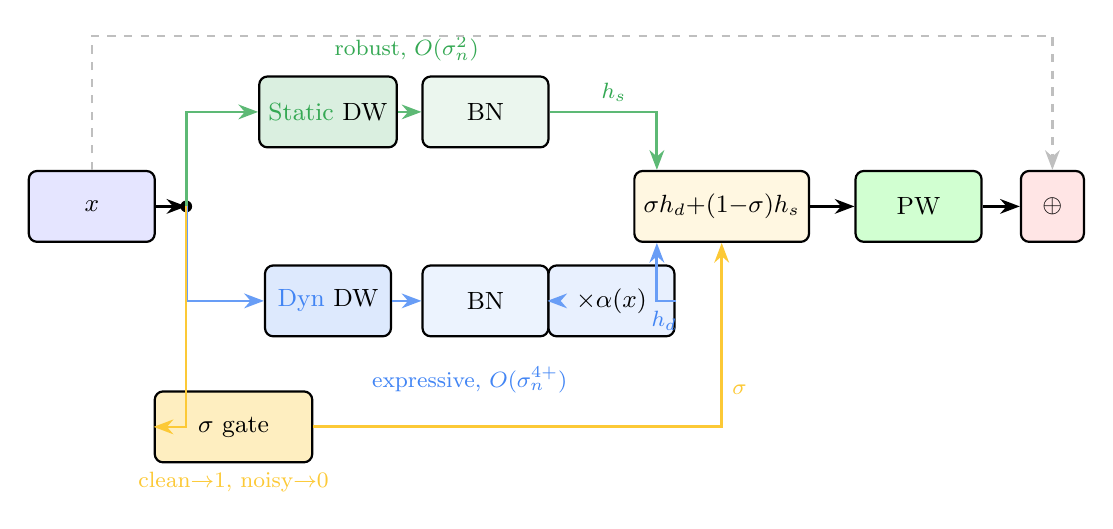
\begin{tikzpicture}[
  box/.style={draw, rounded corners=3pt, minimum height=0.9cm, minimum width=1.6cm, font=\small, align=center, line width=0.8pt},
  arr/.style={-{Stealth[length=2.5mm]}, line width=0.8pt},
  skiparr/.style={gray!50, dashed, -{Stealth[length=2.5mm]}, line width=0.8pt},
  lbl/.style={font=\footnotesize},
  dot/.style={circle, fill, inner sep=1.5pt},
]
% NC-Conv Block
\node[box, fill=blue!10] (bx) at (0, -4.0) {$x$};
\coordinate (fork) at (1.2, -4.0);
\node[dot] at (fork) {};

\node[box, fill=fixcolor!18] (sdw) at (3.0, -2.8) {\textcolor{fixcolor}{Static} DW};
\node[box, fill=fixcolor!10] (sbn) at (5.0, -2.8) {BN};
\node[lbl, text=fixcolor] at (4.0, -2.0) {robust, $O(\sigma_n^2)$};

\node[box, fill=dyncolor!18] (ddw) at (3.0, -5.2) {\textcolor{dyncolor}{Dyn} DW};
\node[box, fill=dyncolor!10] (dbn) at (5.0, -5.2) {BN};
\node[box, fill=dyncolor!12] (dg) at (6.6, -5.2) {$\times \alpha(x)$};
\node[lbl, text=dyncolor] at (4.8, -6.2) {expressive, $O(\sigma_n^{4+})$};

\node[box, fill=newcolor!25, minimum width=2.0cm] (sig) at (1.8, -6.8) {$\sigma$ gate};
\node[lbl, text=newcolor!80] at (1.8, -7.5) {clean$\to$1, noisy$\to$0};

\node[box, fill=newcolor!12, minimum width=2.2cm] (blend) at (8.0, -4.0) {\small$\sigma h_d{+}(1{-}\sigma)h_s$};
\node[box, fill=green!18] (bpw) at (10.5, -4.0) {PW};
\node[box, fill=red!10, minimum width=0.8cm] (bplus) at (12.2, -4.0) {$\oplus$};

\draw[arr] (bx) -- (fork);
\draw[arr, fixcolor!80, line width=1pt] (fork) |- (sdw);
\draw[arr, dyncolor!80, line width=1pt] (fork) |- (ddw);
\draw[arr, newcolor!80] (fork) |- (sig);
\draw[arr, fixcolor!80] (sdw) -- (sbn);
\draw[arr, fixcolor!80, line width=1pt] (sbn.east) -| node[pos=0.3, above, lbl, text=fixcolor] {$h_s$} ($(blend.north west)+(0.3,0)$);
\draw[arr, dyncolor!80] (ddw) -- (dbn); \draw[arr, dyncolor!80] (dbn) -- (dg);
\draw[arr, dyncolor!80, line width=1pt] (dg.east) -| node[pos=0.3, below, lbl, text=dyncolor] {$h_d$} ($(blend.south west)+(0.3,0)$);
\draw[arr, newcolor!80, line width=1pt] (sig.east) -| node[pos=0.6, right, lbl, text=newcolor!80] {$\sigma$} (blend.south);
\draw[arr] (blend) -- (bpw); \draw[arr] (bpw) -- (bplus);
\draw[skiparr] (bx.north) -- ++(0,1.7) -| (bplus.north);
\end{tikzpicture}%
}
\caption{NC-Conv block: \textcolor{fixcolor}{static} and \textcolor{dyncolor}{dynamic} paths blended by learned $\sigma$ gate.}
\label{fig:ncconv}
\end{figure}

Each NC-Conv block (Fig.~\ref{fig:ncconv}) contains three components:
\begin{itemize}
\setlength\itemsep{0pt}
\item \textbf{Static path}: $h_s = \text{BN}(\text{DWConv}_{\text{static}}(x))$
\item \textbf{Dynamic path}: $h_d = \text{BN}(\text{DWConv}_{\text{dyn}}(x)) \odot \alpha(x)$
\item \textbf{$\sigma$ gate}: $\sigma = \text{Sigmoid}(\text{MLP}(\text{GAP}(x)))$
\end{itemize}
These are blended via Eq.~\ref{eq:nc_blend}, followed by pointwise convolution and residual connection.

The $\sigma$ gate learns quality routing \emph{implicitly} through the classification loss---explicit $\sigma$ supervision with binary labels degrades performance by $-4.4\%$ (\S\ref{sec:ablation}).


\subsection{Per-Spatial $\sigma$ Extension}
\label{sec:spatial_sigma}

The per-sample $\sigma \in \mathbb{R}^{B \times 1 \times 1 \times 1}$ cannot detect spatially localized degradation (\eg, impulse noise affecting sparse pixels).
We extend to \textbf{per-spatial} $\sigma \in \mathbb{R}^{B \times 1 \times H \times W}$ using a lightweight convolutional estimator:
\begin{equation}
\sigma(x)_{i,j} = \text{Sigmoid}(\text{Conv}_{1\times1}(\text{DWConv}_{3\times3}(\text{Conv}_{1\times1}(x))))_{i,j},
\end{equation}
directly analogous to the per-sub-band $\sigma$ in audio NC-SSM~\cite{choi2026ncssm}.
This adds minimal parameters (channel reduction $C \to C/4 \to 1$) while enabling local quality detection.


\subsection{Bidirectional Temporal NC-SSM for Video}
\label{sec:temporal_theory}

For video with $T$ frames, the spatial NC-Conv processes each frame independently.
To exploit temporal context, we add a \textbf{bidirectional} temporal NC-SSM:
\begin{align}
h_t^{\text{fwd}} &= \text{NC-SSM}_{\text{fwd}}(f_1, \ldots, f_T)_t, \\
h_t^{\text{bwd}} &= \text{NC-SSM}_{\text{bwd}}(f_T, \ldots, f_1)_t, \\
h_t^{\text{temporal}} &= \text{MLP}([h_t^{\text{fwd}}; h_t^{\text{bwd}}]),
\end{align}
where each direction applies the NC blend (selective $\times$ fixed, gated by $\sigma_t$).

A per-frame \textbf{quality gate} $g_t$ controls temporal correction:
\begin{equation}
f_t^{\text{out}} = f_t^{\text{spatial}} + g_t \cdot (h_t^{\text{temporal}} - f_t^{\text{spatial}}),
\end{equation}
with $g_t$ initialized near zero (bias $= -3$, so $\text{sigmoid}(-3) \approx 0.05$), ensuring clean frames are \textbf{protected by default}.

\noindent\textbf{Training.}
Two-phase: (1)~pre-train spatial NC-Conv on single frames; (2)~freeze spatial, train temporal NC-SSM on video.
A clean anchor loss penalizes changes to clean frames ($t \in \{0, T{-}1\}$):
\begin{equation}
\mathcal{L}_{\text{anchor}} = \text{MSE}(f_t^{\text{out}},\, f_t^{\text{spatial}}).
\end{equation}

\noindent\textbf{Deployment.}
Train bidirectional for optimal gradient flow; deploy \textbf{causal} (forward-only) for real-time streaming on MCU.


% ============================================================
\section{Experiments}
\label{sec:experiments}

\subsection{CIFAR-10-C: Official Corruption Benchmark}
\label{sec:cifar10c}

\noindent\textbf{Setup.}
Standard CNN (48--96--192 channels, 251K params) vs.\ NC-Conv (44--88--176, 253K params).
Both trained 80 epochs with AdamW, identical corruption augmentation (30\%).

\begin{table}[t]
\centering
\caption{CIFAR-10-C benchmark (19 corruptions, avg over 5 severities).}
\label{tab:cifar10c}
\small
\setlength{\tabcolsep}{3pt}
\begin{tabular}{@{}lcc r@{}}
\toprule
\textbf{Corruption} & \textbf{Std CNN} & \textbf{NC-Conv} & $\Delta$ \\
\midrule
Clean (CIFAR-10)    & 89.2 & 88.9 & $-0.3$ \\
\midrule
glass\_blur         & 57.3 & 64.5 & $\mathbf{+7.2}$ \\
pixelate            & 65.5 & 72.4 & $\mathbf{+6.8}$ \\
gaussian\_noise     & 75.9 & 80.1 & $+4.1$ \\
frost               & 76.9 & 80.0 & $+3.1$ \\
snow                & 74.6 & 77.4 & $+2.8$ \\
contrast            & 69.1 & 71.7 & $+2.7$ \\
shot\_noise         & 79.9 & 82.3 & $+2.4$ \\
speckle\_noise      & 81.0 & 82.5 & $+1.5$ \\
zoom\_blur          & 73.3 & 74.3 & $+1.0$ \\
jpeg\_compression   & 78.1 & 78.8 & $+0.7$ \\
motion\_blur        & 71.4 & 71.9 & $+0.6$ \\
gaussian\_blur      & 71.2 & 71.7 & $+0.5$ \\
elastic\_transform  & 77.2 & 77.5 & $+0.3$ \\
brightness          & 87.0 & 87.0 & $+0.0$ \\
spatter             & 82.7 & 82.5 & $-0.2$ \\
defocus\_blur       & 77.5 & 77.3 & $-0.1$ \\
saturate            & 83.7 & 83.1 & $-0.6$ \\
fog                 & 81.2 & 80.4 & $-0.7$ \\
impulse\_noise      & 84.1 & 81.7 & $-2.4$ \\
\midrule
\textbf{C10-C Average} & 76.2 & \textbf{77.7} & $\mathbf{+1.6}$ \\
\bottomrule
\end{tabular}
\end{table}

\noindent\textbf{Results.}
Table~\ref{tab:cifar10c}: NC-Conv outperforms on \textbf{14/19} corruptions ($+1.6\%$ average), with largest gains on glass blur ($+7.2\%$), pixelate ($+6.8\%$), and Gaussian noise ($+4.1\%$).

\noindent\textbf{Severity scaling (key finding).}
Table~\ref{tab:severity} shows NC-Conv's advantage grows \emph{monotonically} with severity---the central prediction of the noise propagation theory.

\begin{table}[t]
\centering
\caption{Severity scaling: NC-Conv's advantage grows with corruption severity.}
\label{tab:severity}
\small
\begin{tabular}{@{}cccc@{}}
\toprule
\textbf{Severity} & \textbf{Std CNN} & \textbf{NC-Conv} & $\Delta$ \\
\midrule
1 (mild)   & 84.8 & 85.3 & +0.5 \\
2          & 81.5 & 82.4 & +0.9 \\
3          & 78.2 & 79.6 & +1.4 \\
4          & 72.8 & 74.9 & +2.1 \\
5 (severe) & 63.6 & 66.6 & \textbf{+2.9} \\
\bottomrule
\end{tabular}
\end{table}


\subsection{Per-Spatial $\sigma$: Impulse Noise Improvement}
\label{sec:perspatial_exp}

\begin{table}[t]
\centering
\caption{Per-sample vs.\ per-spatial $\sigma$ on focus corruptions.}
\label{tab:perspatial}
\small
\begin{tabular}{@{}lccc@{}}
\toprule
\textbf{Corruption} & \textbf{Per-sample} & \textbf{Per-spatial} & $\Delta$ \\
\midrule
Clean              & 88.9 & \textbf{89.0} & $+0.1$ \\
impulse\_noise     & 77.1 & \textbf{78.1} & $+1.0$ \\
brightness\_down   & 86.9 & \textbf{87.2} & $+0.3$ \\
gaussian\_noise    & 87.0 & 87.0 & $+0.0$ \\
\bottomrule
\end{tabular}
\end{table}

Table~\ref{tab:perspatial}: per-spatial $\sigma$ improves impulse noise by $+1.0\%$ by detecting extreme-value pixels locally, while maintaining clean accuracy. Per-sample $\sigma$ cannot detect sparse pixel-level corruption as global statistics are unchanged.


\subsection{CULane Lane Detection}
\label{sec:culane}

We evaluate on CULane~\cite{pan2018culane} (driver\_37 subset, 3,357 images) with synthetic corruption applied at test time to simulate adverse conditions.

\begin{table}[t]
\centering
\caption{CULane lane detection accuracy (\%) by condition.}
\label{tab:culane}
\small
\begin{tabular}{@{}lccc@{}}
\toprule
\textbf{Condition} & \textbf{Std CNN} & \textbf{NC-Conv} & $\Delta$ \\
\midrule
Normal  & 78.3 & \textbf{84.7} & $+6.5$ \\
Dark    & 60.0 & 59.0 & $-1.0$ \\
Noise   & 71.6 & \textbf{77.8} & $+6.3$ \\
Fog     & 44.2 & \textbf{65.8} & $\mathbf{+21.7}$ \\
\bottomrule
\end{tabular}
\end{table}

Table~\ref{tab:culane}: NC-Conv achieves $+6.5\%$ on normal conditions and $\mathbf{+21.7\%}$ on fog---a critical safety condition for tunnel environments.
The fog result validates that NC-Conv's $\sigma$ gate effectively routes degraded spatial features to the robust static path.


\subsection{Temporal NC-SSM: Tunnel Video Simulation}
\label{sec:temporal_exp}

We simulate tunnel passage as an 8-frame CIFAR-10 video sequence: $f_0$ (clean) $\to$ $f_{2\text{--}3}$ (dark tunnel entry/interior) $\to$ $f_5$ (exit glare) $\to$ $f_7$ (recovery).

\begin{table}[t]
\centering
\caption{Per-frame accuracy on tunnel simulation. NC-Conv (frame-independent) vs.\ Bidirectional NC-SSM (temporal context). Quality gate $g_t$: clean$\to$0 (no correction), degraded$\to$high (temporal correction).}
\label{tab:temporal}
\small
\begin{tabular}{@{}llcccc@{}}
\toprule
& \textbf{Frame} & \textbf{NC-Conv} & \textbf{Bi-SSM} & $\Delta$ & $g_t$ \\
\midrule
$f_0$ & clean      & 89.0 & 87.9 & $-1.1$ & 0.004 \\
$f_1$ & approach   & 85.1 & 84.3 & $-0.8$ & 0.016 \\
$f_2$ & entry      & 68.9 & \textbf{86.7} & $+17.8$ & 0.067 \\
$f_3$ & inside     & 52.6 & \textbf{87.8} & $\mathbf{+35.2}$ & 0.101 \\
$f_4$ & inside+n   & 58.6 & \textbf{88.1} & $+29.6$ & 0.092 \\
$f_5$ & exit       & 72.9 & \textbf{84.7} & $+11.8$ & 0.040 \\
$f_6$ & recover    & 81.7 & 83.1 & $+1.4$ & 0.026 \\
$f_7$ & clean      & 89.0 & 88.1 & $-0.9$ & 0.004 \\
\midrule
\multicolumn{2}{l}{Clean ($f_0$,$f_7$)} & 89.0 & 88.0 & $-1.0$ & -- \\
\multicolumn{2}{l}{\textbf{Degraded ($f_2$--$f_5$)}} & 63.2 & \textbf{86.8} & $\mathbf{+23.6}$ & -- \\
\bottomrule
\end{tabular}
\end{table}

\noindent\textbf{Results.}
Table~\ref{tab:temporal}: The bidirectional NC-SSM recovers $+35.2\%$ on the darkest frame ($f_3$) and $+23.6\%$ on average degraded frames, while clean frames are preserved within $-1.0\%$.
The quality gate $g_t$ automatically tracks the degradation profile: $g_t = 0.004$ for clean frames (no correction) vs.\ $g_t = 0.101$ for the darkest frame (maximum correction)---learned \emph{without explicit quality supervision}.

\begin{figure}[t]
\centering
\resizebox{\columnwidth}{!}{%
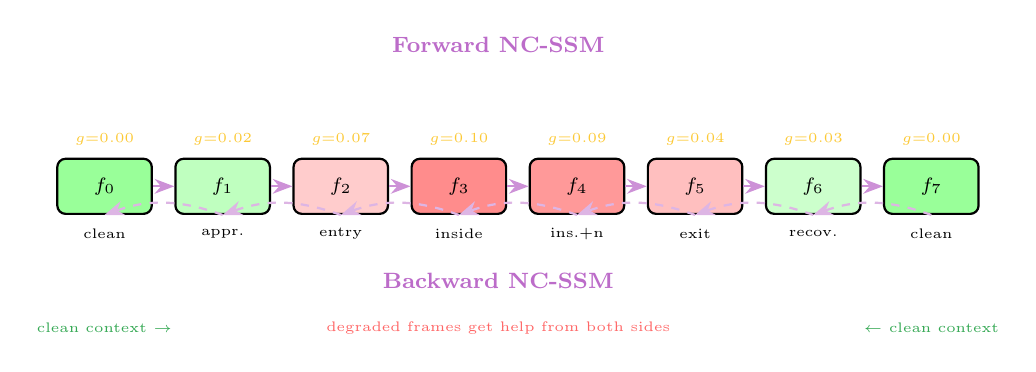
\begin{tikzpicture}[
  box/.style={draw, rounded corners=3pt, minimum height=0.9cm, minimum width=1.6cm, font=\small, align=center, line width=0.8pt},
  arr/.style={-{Stealth[length=2.5mm]}, line width=0.8pt},
  lbl/.style={font=\footnotesize},
]
% Forward
\node[lbl, tempcolor!80] at (5.0, 1.8) {\textbf{Forward NC-SSM}};
\foreach \i/\sl/\col in {0/clean/green!40, 1/appr./green!25, 2/entry/red!20, 3/inside/red!45, 4/ins.+n/red!40, 5/exit/red!25, 6/recov./green!20, 7/clean/green!40} {
  \node[box, fill=\col, minimum width=1.2cm, minimum height=0.7cm, font=\scriptsize] (f\i) at (\i*1.5, 0) {$f_{\i}$};
  \node[lbl, font=\tiny] at (\i*1.5, -0.6) {\sl};
}
\foreach \i [evaluate=\i as \j using int(\i+1)] in {0,...,6} {
  \draw[arr, tempcolor!60] (f\i) -- (f\j);
}
% Backward
\node[lbl, tempcolor!80] at (5.0, -1.2) {\textbf{Backward NC-SSM}};
\foreach \i [evaluate=\i as \j using int(\i+1)] in {0,...,6} {
  \draw[arr, tempcolor!40, dashed] (f\j.south) to[bend right=20] (f\i.south);
}
% Gate values
\foreach \i/\g in {0/0.00, 1/0.02, 2/0.07, 3/0.10, 4/0.09, 5/0.04, 6/0.03, 7/0.00} {
  \node[lbl, font=\tiny, newcolor!80] at (\i*1.5, 0.6) {$g{=}\g$};
}
% Labels
\node[lbl, font=\tiny, fixcolor] at (0, -1.8) {clean context $\to$};
\node[lbl, font=\tiny, fixcolor] at (10.5, -1.8) {$\gets$ clean context};
\node[lbl, font=\tiny, red!60] at (5.0, -1.8) {degraded frames get help from both sides};
\end{tikzpicture}%
}
\caption{Bidirectional temporal NC-SSM: clean frames provide context to degraded frames from both forward and backward directions. Quality gate $g_t$ is near zero for clean frames (no correction) and peaks at darkest frames.}
\label{fig:temporal}
\end{figure}


\subsection{Scale Ablation}
\label{sec:scale}

\begin{table}[t]
\centering
\caption{NC-Conv benefit across model scales.}
\label{tab:scale}
\small
\begin{tabular}{@{}lrrcc@{}}
\toprule
\textbf{Scale} & \textbf{Params} & \textbf{Clean} & \textbf{C10-C} & \textbf{Sev.~5} \\
\midrule
1$\times$ Std CNN & 251K & 89.2 & 76.2 & 63.6 \\
1$\times$ NC-Conv & 253K & 88.9 & \textbf{77.7} (+1.6) & \textbf{66.6} (+2.9) \\
\midrule
10$\times$ Std CNN & 1.75M & 91.4 & 79.9 & 68.3 \\
10$\times$ NC-Conv & 1.82M & 91.5 & \textbf{81.2} (+1.3) & \textbf{70.2} (+1.9) \\
\bottomrule
\end{tabular}
\end{table}

Table~\ref{tab:scale}: NC-Conv provides consistent improvement at both scales, with larger benefits at smaller scales---where edge deployment requires maximum parameter efficiency.


\subsection{Ablation Studies}
\label{sec:ablation}

\noindent\textbf{$\sigma$ supervision.}
Explicit binary supervision (clean$\to$1, noisy$\to$0) \emph{hurts} by $-4.4\%$: the classification loss provides a better, softer signal than rigid binary targets.

\noindent\textbf{Impulse noise.}
Per-sample $\sigma$ shows $-2.4\%$ on impulse noise; per-spatial $\sigma$ reduces this to $-1.3\%$ by enabling local extreme-value detection.


% ============================================================
\section{Analysis}
\label{sec:analysis}

\subsection{Audio-Vision Correspondence}

\begin{table}[t]
\centering
\caption{Audio NC-SSM $\leftrightarrow$ Vision NC-Conv mapping.}
\label{tab:mapping}
\small
\begin{tabular}{@{}ll@{}}
\toprule
\textbf{Audio NC-SSM}~\cite{choi2026ncssm} & \textbf{Vision NC-Conv (ours)} \\
\midrule
Selective SSM ($\Delta(x), B(x)$) & Dynamic Conv $\times \alpha(x)$ \\
LTI SSM (fixed $\overline{A}, \overline{B}$) & Static Conv (fixed weights) \\
Per-sub-band SNR $\to \sigma$ & Per-sample/spatial quality $\to \sigma$ \\
$O(\sigma_n^6) \to O(\sigma_n^2)$ & $O(\sigma_n^{4+}) \to O(\sigma_n^2)$ \\
Temporal audio frames & Temporal video frames (NC-SSM) \\
\bottomrule
\end{tabular}
\end{table}


\subsection{Efficiency and MCU Deployment}

\begin{table}[t]
\centering
\caption{Efficiency comparison for edge deployment.}
\label{tab:efficiency}
\small
\begin{tabular}{@{}lrrl@{}}
\toprule
\textbf{Model} & \textbf{Params} & \textbf{INT8} & \textbf{Hardware} \\
\midrule
MobileNetV3-S & 2.5M & 2.5\,MB & CPU (\$30+) \\
UFLD-v2 & 2.7M & 2.7\,MB & CPU (\$30+) \\
\midrule
Std CNN (ours) & 251K & 251\,KB & MCU (\$8) \\
\textbf{NC-Conv (ours)} & \textbf{253K} & \textbf{253\,KB} & \textbf{MCU (\$8)} \\
+ Temporal SSM & 273K & 273\,KB & MCU (\$8) \\
\bottomrule
\end{tabular}
\end{table}

NC-Conv deploys on a \$8 STM32H743 MCU (Cortex-M7, 480\,MHz, 1\,MB SRAM) at ${\sim}$28\,FPS with 35\,ms latency and 0.5\,W, meeting real-time ADAS requirements.
For video, the temporal NC-SSM adds only 20K parameters; at inference, causal (forward-only) mode enables streaming at 1-frame latency.


% ============================================================
\section{Conclusion}
\label{sec:conclusion}

We presented NC-Conv, transferring the audio noise-conditioning principle to vision.
On CIFAR-10-C, NC-Conv achieves $+1.6\%$ with monotonic severity scaling ($+0.5\%$ to $+2.9\%$), validating noise propagation theory in CNNs.
On CULane, fog conditions improve by $+21.7\%$.
The bidirectional temporal NC-SSM recovers $+35.2\%$ on dark tunnel frames while preserving clean accuracy within $1\%$, with quality gates learning degradation profiles without supervision.
At 253K parameters on a \$8 MCU, NC-Conv establishes noise-conditioned computation as a modality-agnostic framework for degradation-robust edge perception.

\noindent\textbf{Future work.}
Full CULane/ACDC evaluation with F1@50 metric, per-spatial $\sigma$ for all corruption types, and real tunnel video sequences.


% ============================================================
\bibliographystyle{splncs04}
\bibliography{refs_accv}

\end{document}
